\documentclass{article}
\usepackage[utf8]{inputenc}
\usepackage{physics}
\usepackage{listings}
\usepackage{graphicx}
\usepackage{flexisym}
\usepackage[export]{adjustbox}

%%%%%%%%%%%%%%%%%%%%%%%%%%%%%%%%%%
\documentclass[14pt, a4paper, twoside]{article}
\usepackage[margin=1in,bindingoffset=5.5mm,heightrounded]{geometry}
\usepackage[T1]{fontenc}
\usepackage{indentfirst}
%\vspace*{36 pt}
\title{Applied Mathematics  Assignment 01 \\ TW244 Applied Differential Equations}
\author{https://github.com/BhekimpiloNdhlela/TW244AppliedDifferentialEquations \\ \\ Bhekimpilo Ndhlela (18998712)}
\date{11 May 2018}
\begin{document}
\maketitle
\pagebreak

\section*{Problem 1}
\subsection*{Question a.)}
\begin{center}
\[\frac{dP}{dt} = P^3 - 4P^2 + 4P = P(P^2 - 4P + 4)\] \[\frac{dP}{dt} = P(P -2)^2\] \\  \textbf{let: $\frac{dP}{dt} = 0 = P(P - 2)^2 $ therefore: $P = 0$ or $P = 2$} 
\end{center}

\subsection*{Question b.)}
\begin{center}
\[\frac{d^2P}{dt^2} = \frac{d}{dt}(P^3 - 4P^2 + 4P) = 3P^2\frac{dP}{dt} - 8P\frac{dP}{dt} + 4\frac{dP}{dt}\]
\[\frac{d^2P}{dt^2} = \frac{dP}{dt}(3P^2 - 8P + 4) = P(P -2)^2(3P^2 - 8P + 4)\]
\[\frac{d^2P}{dt^2} =  P(P -2)^3(3P - 2)\] \textbf{let : $\frac{d^2P}{dt^2} = 0 = P(P -2)^3(3P - 2)$ therefore: $P = 0$, $P = 2$ or $P = \frac{2}{3}$}
\end{center}
\textbf{Increasing: $P > 0$ \\ }
\textbf{Decreasing: $P < 0$ \\}
\textbf{Concave Up: $P > 2$(not of interest) and $0 < P < \frac{2}{3}$ \\}
\textbf{Concave Down: $P < 0$ and $ \frac{2}{3} < P < 2$}

\subsection*{Question c.) and d.)}
\pagebreak
\subsection*{Question e.)}
\begin{figure}[h!]
  \centering
  \begin{subfigure}{\linewidth}
    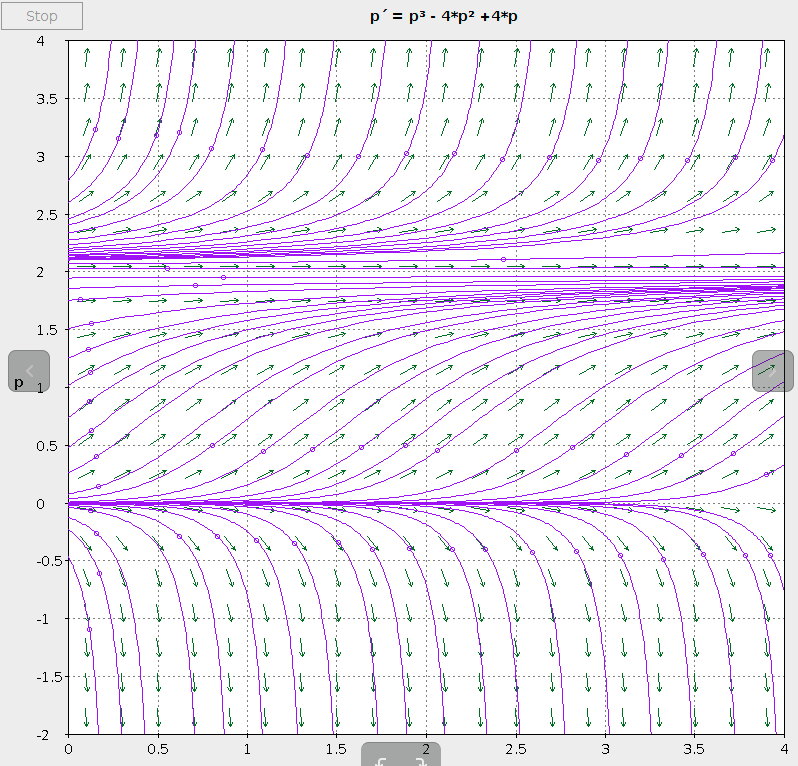
\includegraphics[width=\linewidth]{problem1e.png}
    \caption{Solution Curve with the aid of dfield8}
  \end{subfigure}
\end{figure}
\pagebreak

\section*{Problem 2}
\subsection*{Question a.)}
\begin{center}
\textbf{Required to Show: $y(x) = ce^{-e^{-x}}$ given that: $\frac{dy}{dx} = e^{-x}y$ \\} \textbf{\\ \\by the separation of variables the following holds true: }
\[\frac{dy}{dx} = e^{-x}y \implies \int \frac{1}{y}dy = \int e^{-x}dx\]
\[ \ln{y} = -e^{-x} + k \implies y = e^{-e^{-x} + k}\]
\[y = e^ke^{-e^{-x}}\]
\\ \\ \textbf{let: $e^k = c \implies y = ce^{-e^{-x}}$}
\end{center}

\subsection*{Question b.)}
\begin{center}
\textbf{$\frac{dy}{dx} = e^{-x}y$ where: $y(0) = 1$} 
\[y = e^{-e^{-x} + k} \implies y(0) = 1 = e^{-e^{0} + k} \]
\[1 = e^{-1 + k} \implies 1 = \frac{e^{k}}{e} \implies e = e^k \implies k = 1\]
\[y(x) = e^{-e^{-x} + 1} = e^{1 -e^{-x}}\]

\subsection*{Python Source Code}
\begin{lstlisting}[language=Python]
X = linspace(0, 4, 1000)
y = array([ exp(1-exp(-x)) for x in X])
plt.title('Plot of function f(x) = exp(1-exp(-x))')
plt.xlabel('x = linspace(0, 4, 1000)')
plt.ylabel('f(x) = exp(1-exp(-x))')
plt.plot(X, y, '-k', linewidth=4)
plt.show()
\end{lstlisting}
\pagebreak
\begin{figure}[h!]
  \centering
  \begin{subfigure}{\linewidth}
    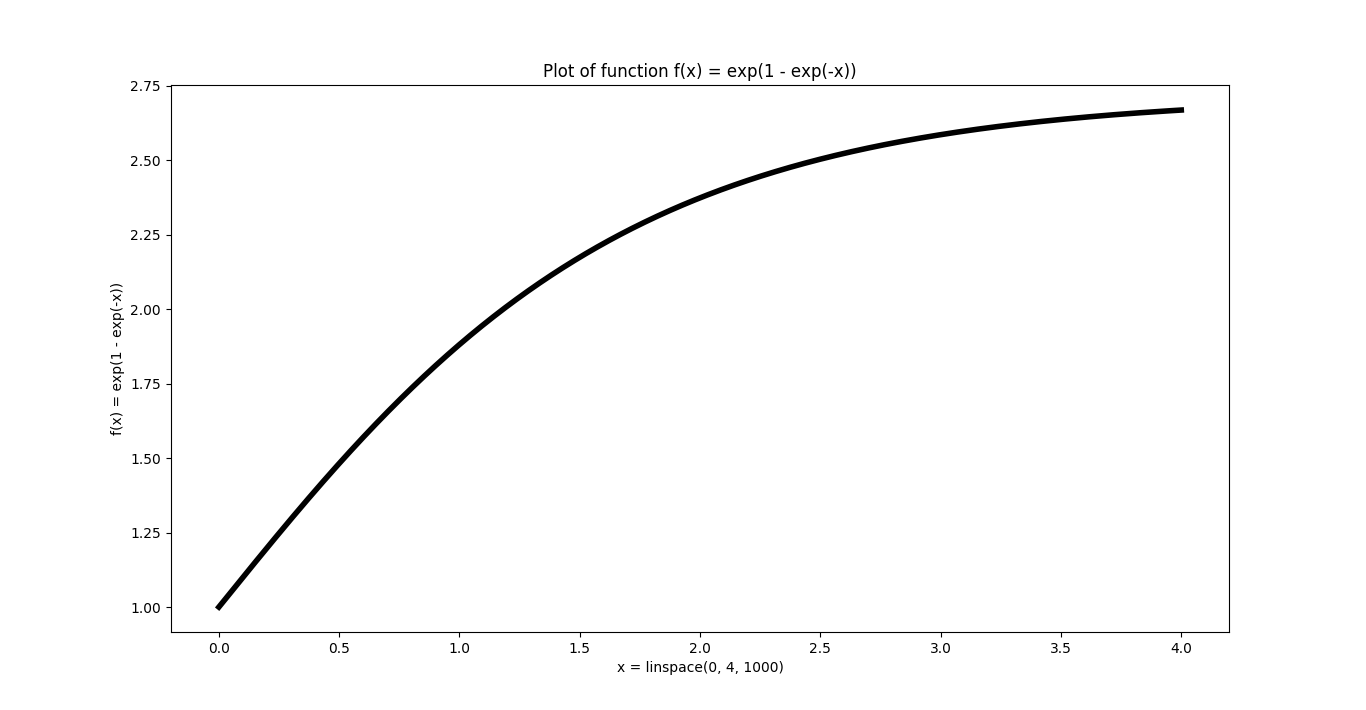
\includegraphics[width=\linewidth]{Figure_2-1.png}
    \caption{Analytical Solution}
  \end{subfigure}
\end{figure}
\end{center}
\pagebreak




\subsection*{Question c.)}
\subsection*{Python Source Code For Problem 2c.)}
\begin{lstlisting}[language=Python]
def eulers_method(f, I, y0=1.0,(a,b)=(0.0,4.0), h=1.0):
    X = array([0.0, 1.0, 2.0, 3.0, 4.0])
    W = array([y0, 0.0, 0.0, 0.0, 0.0])

    for i in xrange(int(a), int(b)):
        W[i+1] = W[i] + h * f(X[i], W[i])
    absolute_error(W, X, 'Euler\'s Method')
    
f = lambda x, y: exp(-x) * y    # f(x, y) = y DE
I = lambda x: exp(1 - exp(-x))  # Exact Solution
eulers_method(f, I)
\end{lstlisting}

\begin{figure}[h!]
  \centering
  \begin{subfigure}{\linewidth}
    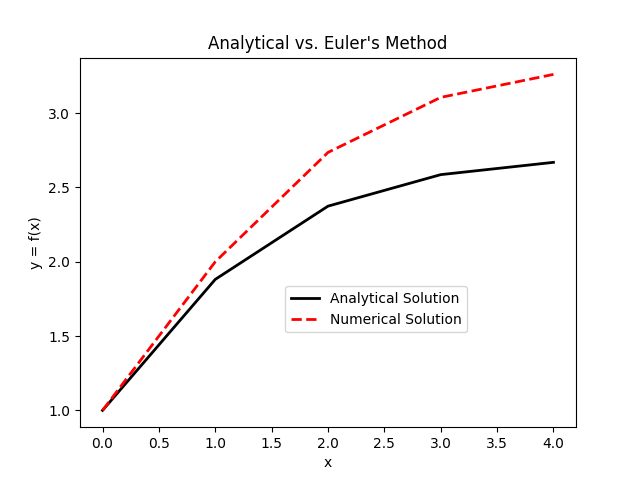
\includegraphics[width=\linewidth]{Figure_2-2.png}
    \caption{Comparison of Analytical Solution and Euler's Method, when: $h = 1$}
  \end{subfigure}
\end{figure}

 \begin{center}
\begin{tabular}{ |c|c|c|c| } 
 \hline \hline
    $x$    &  $w$           &  $y$ & Absolute Error = $|X_c - X|$ \\ 
 \hline \hline       
    0      & 1.0000000000 & 1.0000000000 & 0.0000000000\\
 \hline
    1      & 2.0000000000 &   1.8815963875  &   0.1184036125\\
 \hline
    2      & 2.7357588823 &   2.3742099197  &   0.3615489626\\
 \hline
    3      & 3.1060035856 &   2.5862602973  &   0.5197432882\\
 \hline
    4      & 3.2606423984 &   2.6689479302  &    0.5916944683\\
 \hline
\end{tabular}
\end{center}
\pagebreak

\subsection*{Question d.)}
\subsection*{Python Source Code For Problem 2d.)}
\begin{lstlisting}[language=Python]
def modified_eulers_method(f, I, y0=1.0,(a,b)=(0.0,4.0), h=1.0):
    X = array([0.0, 1.0, 2.0, 3.0, 4.0])
    W = array([y0, 0.0, 0.0, 0.0, 0.0])

    for i in xrange(int(a), int(b)):
        temp = W[i] + h*f(X[i], W[i])
        W[i+1] = W[i] + (h/2.0)*(f(X[i], W[i]) + f(X[i+1], temp))
    absolute_error(W, X, 'Improved Euler\'s Method')

f = lambda x, y: exp(-x) * y    # f(x, y) = y DE
I = lambda x: exp(1 - exp(-x))  # Exact Solution
modified_eulers_method(f, I)
\end{lstlisting}

\begin{figure}[h!]
  \centering
  \begin{subfigure}{\linewidth}
    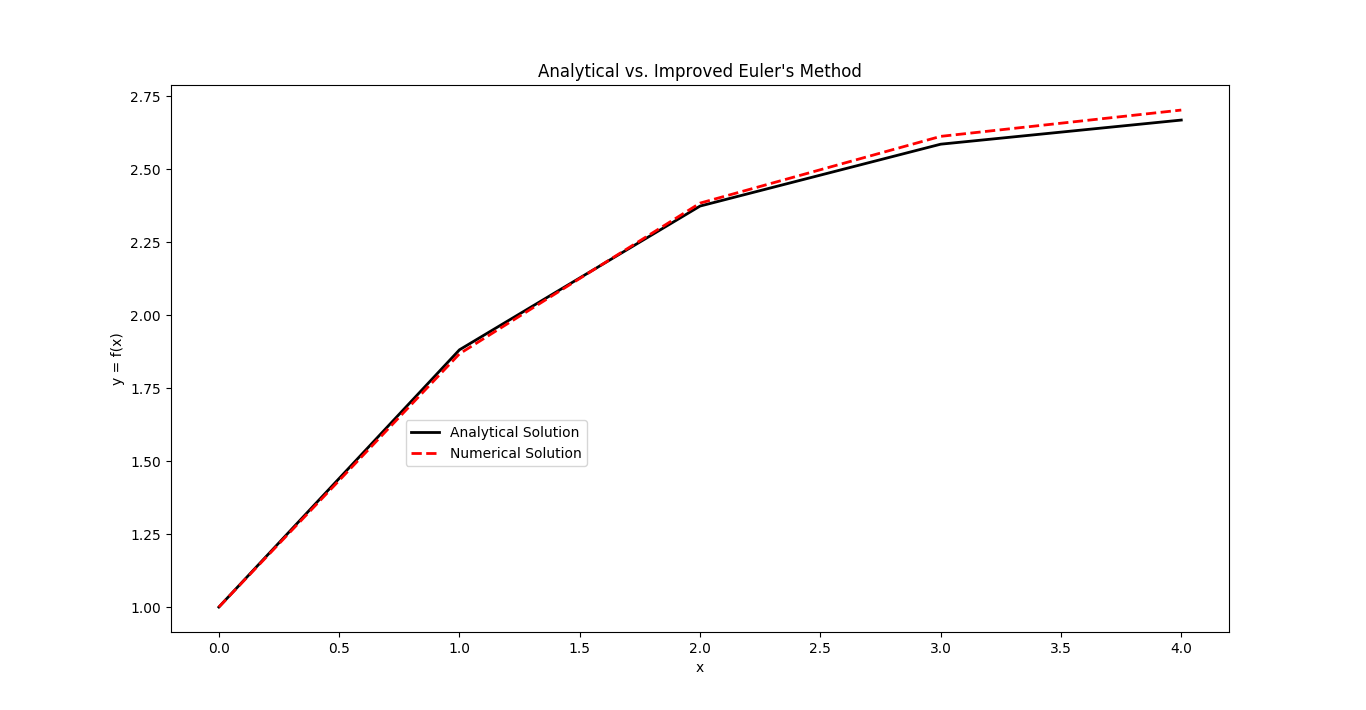
\includegraphics[width=\linewidth]{Figure_2-3.png}
    \caption{Comparison of Analytical Solution and Improved Euler's Method, when: $h = 1$}
  \end{subfigure}
\end{figure}
 \begin{center}
\begin{tabular}{ |c|c|c|c| } 
 \hline \hline
    $x$    &  $w$           &  $y$ & Absolute Error = $|X_c - X|$ \\ 
 \hline \hline       
    0   & 1.0000000000 & 1.0000000000 & 0.0000000000\\
 \hline
    1   & 1.8678794412 & 1.8815963875 & 0.0137169464\\
 \hline
    2   & 2.3843497810 & 2.3742099197 & 0.0101398613\\
 \hline
    3   & 2.6130808115 & 2.5862602973 & 0.0268205142\\
 \hline
    4   & 2.7032511609 & 2.6689479302 & 0.0343032307\\
 \hline
\end{tabular}
\end{center}
\pagebreak

\subsection*{Utility Functions for Problem 2c and 2d.)}
\begin{lstlisting}[language=Python]
def absolute_error(W, X, label, debug=True):
    Y = array([ I(n) for n in xrange(len(W))])
    abs_err = array([abs(ya - yc) for ya, yc in zip(Y, W)])
    if debug is True:
        print(label)
        for i , (err, w) in enumerate(zip(abs_err, W)):
            print 'x = ', i, '\t\tw = {:.10f} \ty = {:.10f}\terr = {:.10f}'.format(w, Y[i], abs_err[i])
    plot_comparison_func(Y, W, X, label)

def plot_comparison_func(Y, W, x, lbl):
    plt.title('Analytical vs. ' + lbl)
    plt.xlabel('x')
    plt.ylabel('y = f(x)')
    plt.plot(x, Y, '-k', linewidth=2, label='Analytical Solution')
    plt.plot(x, W, '--r', linewidth=2, label='Numerical Solution')
    plt.legend(bbox_to_anchor=(.4, .4))
    plt.show()
    
f = lambda x, y: exp(-x) * y    # f(x, y) = y DE
I = lambda x: exp(1 - exp(-x))  # Exact Solution
eulers_method(f, I)
modified_eulers_method(f, I)
\end{lstlisting}

\pagebreak


\subsection*{Question e.)}
\begin{figure}[h!]
  \centering
  \begin{subfigure}{\linewidth}
    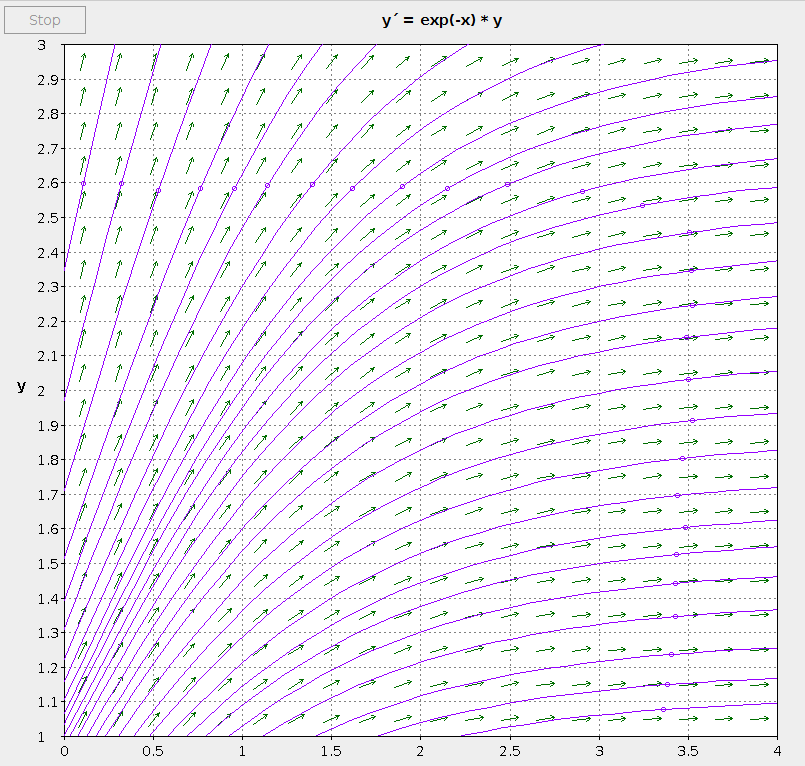
\includegraphics[width=\linewidth]{problem2e.png}
    \caption{Solution Curve with the aid of dfield8}
  \end{subfigure}
\end{figure}
\end{document}